\section{What improved, and where the frontier stands}\label{sec:frontier}

Table~\ref{tab:improvements} collects the measured improvements of the
programme on the boundary each was measured on. Ratios are
baseline/candidate; ``stage'' means one oracle call or one solver run;
``complete'' means a verified discrete logarithm with the stated phases.

\begin{table}[p]
\centering\small
\caption[]{Measured improvements, July--October 2026. Class: E =
\cls{engineering}, A = \cls{accounting}. Boundary: St = stage,
Cx = complete solve outside ecbench, Cold = ecbench cold one-target $S$,
On = online window after retained set-up. Sources: Appendix~\ref{app:artefacts}.}
\label{tab:improvements}
\begin{tabularx}{\linewidth}{@{}>{\raggedright}Xllr>{\raggedright\arraybackslash}p{3.0cm}@{}}
\toprule
Change & Bnd. & Cl. & Ratio & Scope \\
\midrule
\multicolumn{5}{@{}l}{\emph{Decomposition oracle: root finding}}\\
$\Sem3$ roots, binary pair table vs matrix F4 & St & E & $383$--$1{,}535$ & $\FF_{2^9}$, $\FF_{2^{13}}$, $m=2$ \\
$\Sem3$ roots, prime vs \texttt{groebner\_f4} & St & E & $3.5$--$4.7{\cdot}10^4$ & 16--24-bit, $\abs\Fb=6$ \\
$\Sem3$ roots vs Buchberger, NIST curves & St & E & $3{,}021$--$5{,}802$ & P-192\ldots P-521 \\
\texttt{rf-mitm} vs PS-0 oracle & St & E & $3{,}007$--$115{,}160$ & binary $\ell=8..14$ \\
Root-finding DLP vs msolve DLP & Cx & E & $50$--$105$ & 16--24-bit prime \\
Pair-table DLP vs F4 DLP & Cx & E & $122$ & binary $n=23$ (F4 wins $n\le13$) \\
Pair table vs subtraction & Cold & E & $53.0$ & 20-bit prime (bounded) \\
Frobenius pair table vs subtraction & Cold & E & $17.5$ & Koblitz $n=17$, priced \\
Root-finding K13 arm, first to best & Cold & E & $1.69$ & $38.82\to22.97$, across sessions \\
Windowed $m=3$ scan & Cold & E & $1.21$ & $[1.16,1.28]$ \\
Negfold root finding vs XOR-priced F4 & Cold & E & $18.3$ & $[15.6,21.3]$, K13 \\
Dense root index K1798 vs K1500 (probes) & On & E & $1.77$ & $n=83$, one point \\
Pair-table size 64 vs 32 abscissae & Cold & E & $1.20$ & $[1.04,1.43]$ \\
\addlinespace
\multicolumn{5}{@{}l}{\emph{Gr\"obner engines}}\\
Inherited vs matrix F4 (matrix work) & St & E & $198.6$--$222.1$ & K13, R13 \\
F5 vs matrix F4 (word XORs) & St & E & $1.55$--$1.56$ & K13, R13 \\
F6-IC vs inherited F4 (word XORs) & St & E & $1.22$--$1.30$ & $m=13,19$ \\
\texttt{f4\_fp} new vs previous & St & E & $29.8$--$54.1$ & square systems, = msolve \\
Four-Russians routing & St & E & $1.75$--$3.22$ & oracle matrices \\
Eager vs lazy inherited rewrite & St & E & $1.40$--$1.62$ & dim 8--9 \\
Quotient-curve $m=2$ model & St & E & $1.34$--$1.64$ & five cells \\
\addlinespace
\multicolumn{5}{@{}l}{\emph{Factor bases and symmetry}}\\
Compact orbit vs full orbit & Cold & E & $\le1.87$ & Koblitz $n=17$; compact is LB \\
FGHR $D_4$ vs Gaudry $S_4$, $C_4$ & St & E & $47.5$--$48.4$ & $\FF_{269^4}$ \\
\texttt{gaudry\_quartic} solve & St & E & $1.9$--$6.4$ & $d=4..6$ \\
\addlinespace
\multicolumn{5}{@{}l}{\emph{One-target online}}\\
Compact-orbit IC vs strong rho & On & E & $13.94$ & $n=61$, $[9.81,19.13]$, 64 targets \\
\addlinespace
\multicolumn{5}{@{}l}{\emph{Accounting (costs that went up when priced)}}\\
F4 word XORs priced & Cold & A & $1/25.2$ & $16.75\to421.4$, K13 \\
F6-IC batched geometry priced & Cold & A & $1/64.6$--$1/1{,}353$ & $m=13,19$ \\
\bottomrule
\end{tabularx}
\end{table}

\noindent Derived entries: $53.0=1/0.018861$; $17.5=1/0.057047$;
$1.21=1/0.828$ with interval from $[0.783,0.863]$; $18.3=1/0.0545$ with
interval from $[0.047,0.064]$; $1.77=300{,}021.9/169{,}069.8$; $1.20=1/0.830$
with interval from $[0.697,0.962]$; $1.87=18.714/9.985$ (one session; the compact arm's $S$ is a lower bound, so
the ratio is an upper bound); $1.69$ and $25.2$ compare means from different
sessions with different seeds and are descriptive; F5 and F6-IC ratios are
reciprocals of the recorded candidate/baseline word-XOR ratios.

\subsection{Three frontiers}

\paragraph{Cold, one target, set-up included.} Unchanged: generic rho.
Every measured index-calculus arm is above its matched rho
(Figure~\ref{fig:cold}); the closest complete count is root-finding negfold
at $1.55\times$ strong signed-Frobenius rho at $n=13$; the closest
lower-bound arms are $1.08\times$ (compact orbit with a counted Frobenius
table) and $6.97\times$ (matrix F4/F5 against rho-negation at K13).
Prime-field arms are $12$--$239\times$ rho and diverge with size.

\paragraph{Online, after retained set-up.} One admitted point: compact-orbit
IC at Koblitz $n=61$, $13.9\times$ $[9.8,19.1]$ over strong rho on 64
unseen public targets, set-up of about 28\,s excluded (cold median
$83.4\times$ rho). The larger $n=71,73,83$ observations remain exploratory.

\paragraph{Stage.} Moved substantially: the decomposition oracle is two to
five orders of magnitude cheaper than at the start of the programme on the
workloads where root finding applies, the $\FF_p$ F4 is at msolve parity,
the Boolean F4 family is one to two orders of magnitude cheaper in counted
matrix work, and the $k=4$ extension-field solve is $48\times$ cheaper.
None of this, by itself, moves the cold frontier: the stages it leaves
untouched---relation yield, factor-base size, linear algebra, table
set-up---now dominate.

\begin{figure}[t]
\centering
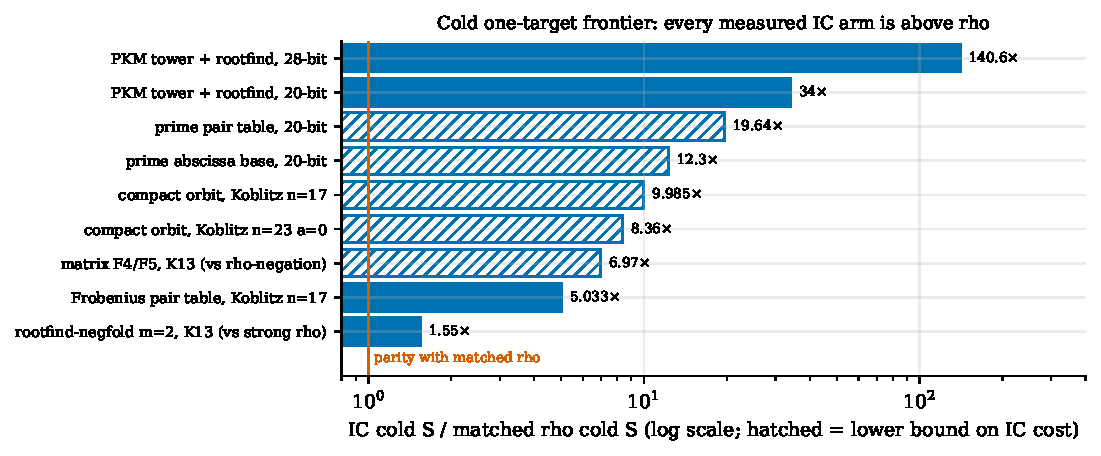
\includegraphics[width=\linewidth]{figures/fig-cold-gap.pdf}
\caption[]{Cold one-target $S$ of index-calculus candidates over their
matched rho arm (each study's own estimator; curves differ, so bars are not
ranked against each other). Hatched: lower bound on IC cost (unpriced
native or solver work). Sources: \art{research/ecbench_frontier_20261013/},
\art{research/ecbench_rootfinding_assessment_20261012/},
\art{research/pkm_tower_ecbench_20261013/},
\art{research/ecbench_rootfind_faster_20261014/}.}
\label{fig:cold}
\end{figure}

\subsection{What would move the cold frontier}

From the frontier synthesis and the problem records: (i) register the
torsion-symmetrised bases and the $n=83$ dense-root engine in ecbench under
immutable method identities and emit cold and online records; (ii) resolve
the inherited-F4 cross-host counter drift before using that counter in a
bound; (iii) run a four-size native challenge against the standing rho
bound---two sizes cannot establish an exponent; (iv) obtain an isolated
cold session at $n=83$ with every set-up phase and retained byte charged;
(v) price F6-IC's batched geometry with a pinned conversion. A result in
the cold domain that beats rho at four sizes would be the first
\cls{advance} of the programme.
